%#!platex -kanji=utf8 hb.tex
\chapter{表紙・タイトルを作成する}
% これはただのダミーテキスト.
% 文字コードを判定するための意味のない文字列.
% これくらい記述すれば大丈夫かな.
% Emacs のくせに生意気な.
% Emacs の分際で自動判別とか.
% Mac OS X のテキストエディッタの文字コード自動判別はうまくいかないぞ.

% 文書の書式・体裁を決定する (geometry, fancyhdr, {px,tx}fonts)
% 表紙を作る (maketitle, titlepage, 自作)

\section{表題}\seclab{maketitle}
%\Z{表題}はその文書が何について書かれたものなのかを示すために
%必要な要素です.通常は\yo{題名},\yo{作者},\yo{日付}を書くのが
%一般的ですからプリアンブルに


\subsection{タイトルを出力する}
\CI{title,author,date,maketitle}%
\begin{usage}
\title{$\<題名>$} 
\author{$\<著者>$}
\date{$\<日付>$}
\maketitle % \begin{document} の後に追加
\end{usage}

%{表題}はその文書が何について書かれたものなのかを示すために
%必要な要素です.通常は\KY{題名} (\Z{title}),\KY{作者} (\Z{author}),
%\KY{日付} (\Z{date}) を書くのが
%一般的ですからプリアンブルに次の三つを書き込みます.

\begin{inout}
\title{\AmSLaTeX の研究}
\author{平賀 源内}
\date{2008/03/31}
\maketitle
\end{inout}


\section{表紙ページを作らずにタイトルを出力する}

\begin{usage}
\documentclass[notitlepage]{jsarticle} 
\end{usage}


\subsection{タイトルを複数行に分ける(副題を付ける)}

\begin{usage}
\title{$\<タイトル>_1$\\ $\<タイトル>_2$\\ $\cdots$ \\ $\<タイトル>_n$} 
\end{usage}

\CI{today}%
\begin{inout}
\title{\AmSLaTeX の研究\\ 
 {\normalsize ―The States of the Art―}}
\author{A. U. Th\'or}
\date{\today}
\maketitle
\end{inout}


\subsection{著者を省略して題名と日付だけ出力する}
\begin{usage}
\title{\\[-$\<空き調整のための数値>$\Cvs]}
\author{}% 空白のままです
\end{usage}
%題名と日付のあいだの空白が広すぎるので,\C{title} 命令の最後に
%負の空きを挿入します.
\begin{inout}
\title{研究室合同親睦会開催のお知らせ\\[-\cvs]}
\author{}
\date{\today}
\maketitle
\end{inout}


\subsection{謝辞・連絡先を追加する}
\CI{thanks}%
\begin{usage}
\author{$\<著者>$\thanks{$\<謝辞・連絡先>$}} 
\end{usage}
\begin{inout}
\title{\AmSLaTeX の研究}
\author{A. U. Th\'or\thanks{author@any.com}}
\date{\today}
\maketitle
\end{inout}

\subsection{複数の著者を追加(連名に)する}
\CI{and}%
\begin{usage}
\author{$\<著者>_1$\and $\<著者>_2$\and $\cdots$ \and $\<著者>_n$} 
\end{usage}
\begin{inout}
\title{Zur Farbenlehre}
\author{A. U. Th\'or \and J. W. von Goethe}
\date{\number\year/\number\month/\number\day}
\maketitle
\end{inout}

%\subsection{著者の所属を著者名の下に追加する}
\subsection{所属・連絡先を著者名の下に表示する}
\begin{usage}
\author{$\<著者>_1$\\ $\<連絡先>_1$ \and 
 $\<著者>_2$\\ $\<連絡先>_2$ \and $\ldots$}  
\end{usage}

\begin{inout}
\title{\AmSLaTeX の研究}
\author{A. U. Th\'or\\ Japan Research Center\\
 author@nrc.org}
\date{\today}
\maketitle 
\end{inout}

\begin{inout}
\title{Zur Farbenlehre}
\author{A. U. Th\'or\\     JRCL\\ author@any.com 
  \and  J. W. von Goethe\\ NRCL\\    goethe@any.com}
\date{\number\year/\number\month/\number\day}
\maketitle
\end{inout}

\section{表紙を別紙で用意してタイトルを出力する}

\begin{usage}
\documentclass[titlepage]{jsarticle} 
\end{usage}


\section{概要を追加する}
\EI{abstract}%
\begin{usage}
\begin{abstract}
 $\<概要をここに記述します>$
\end{abstract} % 2 段組時は \maketitle により出力されます.
\end{usage}

%\begin{usage}
%\documentclass{jsarticle}
%\begin{document}
%\begin{abstract}
% $\<概要をここに記述します>$
%\end{abstract}
%\title{$\<題名>$}
%\author{$\<著者情報>$}
%\date{$\<日付>$}
%\maketitle
%\end{document}
%\end{usage}

%文書の概略が存在すればその文書に何が書かれているのかが大まかに
%分かるので\Z{概要} (\Z{abstract}) を書くのが良いでしょう.
%さすがに1ページの文書には必要ないでしょうが.
%\yo{概要}は\yo{はしがき}とも呼ばれ,文書クラスによって
%出力方法が違います.\cls{(j)article}系ならば
%\Env{abstract}環境を使います.この\env{abstract}環境
%は \Cmd{maketitle} 命令と関わりがあるので概要を出力するために
%は \cmd{maketitle} 命令の後に書きます.


\subsection{1段組みで概要をタイトル下部に出力する}

\begin{inonly}
\author{A. U. Th\'or}
\title{\LaTeXe の研究}
\date{\today}
\maketitle
\begin{abstract}
この文書は\LaTeXe の研究資料である.2008年現在での動向につい
て簡潔にまとめている.詳細は巻末の参考資料を参照して頂きたい.
\end{abstract} 
\end{inonly}
\label{用例:1段組みで概要をタイトル下部に出力する}
\begin{outonly}
\author{A. U. Th\'or}
\title{\LaTeXe の研究}
\date{\today}
\begin{abstract}
 この文書は\LaTeXe の研究資料である.2008年現在での動向について
 も簡潔にまとめている.詳細情報は巻末の参考資料を参照して頂きたい.
\end{abstract}  
\maketitle
\end{outonly}

\subsection{2段組みで概要をタイトル下部に出力する}

\begin{usage}
\author{$\<著者>$} \title{$\<タイトル>$} \date{$\<日付>$}
\begin{abstract}
$\<ここに概要を記述します>$ 
\end{abstract}
\maketitle % abstract環境を\maketitleより前に追加します
\end{usage}

\begin{inonly}
\author{A. U. Th\'or}
\title{\LaTeXe の研究}
\date{\today}
\begin{abstract}
この文書は\LaTeXe の研究資料である.2008年現在の動向について
簡潔にまとめている.詳細は巻末の参考資料を参照して頂きたい.
\end{abstract} 
\maketitle
\end{inonly}
\begin{outonly}
 用例3.8%\ref{用例:1段組みで概要をタイトル下部に出力する}
 の出力例と同様の結果になります.
\end{outonly}


%\subsection{book系のクラスで概要を出力する}
%次に\cls{(j)report}の場合ですが概要専用の環境は用意されてい
%ません.そこで概要を\Z{章立て}すると良いので \Cmd{chapter*} 
%命令を使います.このとき \cmd{chapter}命令にアスタリスク 
%\qu{\texttt*}を付けると目次に見出しを書き出さず,章番号を付け足しません.
%例として次の記述をしてから概要の文章を書きます.

%\begin{intext}
%\chapter*{概要}\addcontentsline{toc}{chapter}{概要}
%\end{intext}

%標準の文書クラスでは
%概要専用のコマンドは定義されていません.用途は異なりますが
%\Hito{奥村}{晴彦}の\Cls{jsbook}には\env{abstract}環境が定義
%されています.これは各章の始めに\yo{この章について}のような
%\kenten{まえがき}を書くときに使われます.

%最後に\cls{(j)book}の場合ですが,これは \Cmd{frontmatter} が宣言
%されているときに \cmd{chapter}命令を使うと余計な手間を省く事ができます.
%具体的には\index{まえがき}%
%次のようにすると目次にも概要を番号なしで書き出します.

%\begin{intext}
%\begin{document} 
%\frontmatter%前付け
%\chapter{まえがき}
%ここに概要やまえがきを書きます.
%\mainmatter%本文
%\chapter{序論}
%\end{intext}

\section{\protect\C{maketitle}命令を使わずに表紙を自作する}
\begin{usage}
\begin{titlepage}
 $\<表紙情報>$
\end{titlepage}
\end{usage}
\E{titlepage}環境を手動で作成します.このとき,以下の命令を使います.
\begin{usage}
\vskip$\<長さ>$ % 長さ分の垂直方向の空きを挿入
\par   % 改行する
\LARGE \Large \large \small % 書体の大きさを変更する
\end{usage}

\subsection{学位論文のような表紙を作成する}
%\C{maketitle} を使わない.大学から提供されていない場合は,手動で以下のよ
%うに調整する方法があります.

%\C{@maketitle}命令を再定義する方法もありますが,
%ここでは \C{maketitle}命令を直接再定義する方法を紹介します.

%この程度でも良いのですが,表紙もまた細かい指定をされる場合
%があります.1から \cmd{maketitle}を作っても良いのですが,一
%刻も早く論文を仕上げなければならないときに,命令を定義して
%は間に合わないかも知れません.そのようなときは断腸の思い
%で \C{titlepage}環境を借用して表紙を作る事もできます.%
%\indindz{表題}{表紙の}\index{表紙の作成}%
%例として \C{maketitle}命令の変更例を紹介します.

\CIS{vskip,cvs,headfont,null,vfill,maketitle,qquad,thispagestyle}%
\CIS{par,let,small,relax,thanks,footnote,footnoterule,normalfont}%
\begin{intext}
\renewcommand{\maketitle}{%
  \begin{titlepage}
    \let \footnotesize \small
    \let \footnoterule \relax
    \let \footnote \thanks
    \null \vskip2 \cvs % ページ上部の空白
    \begin{center}\thispagestyle{empty}%
     {\large\headfont 平成19年度 公立未来大学 卒業論文}%
     \par \vskip 2\cvs
     {\LARGE\headfont ここに表題を書きます}\par 
     \vskip \cvs
     {\Large\normalfont 未来太郎}\par \vskip 2\cvs
     {\small 未来研究学科 \qquad 学籍番号}\par 
     \vskip .5\cvs
     {\small 指導教員 \qquad 北海太郎}\par \vskip \cvs
     {提出日 2008/03/30}\par \vskip 3\cvs
     {\Large\headfont English Title}\par 
     {\large by}\par 
     {\large Your Name}\par \vskip \cvs
     {BA Thesis at Future University, 2007}\par 
     \vskip \cvs
     {Advisor: Prof.~Taro Hokkai}\par \vskip \cvs
     {Dept.~of Future Research}\par 
     {Future University}\par
     {February 2008}%
    \end{center}%
    \vfill \null
  \end{titlepage}%
}
\end{intext}


\begin{figure}[htbp]
 \begin{center}
  \fbox{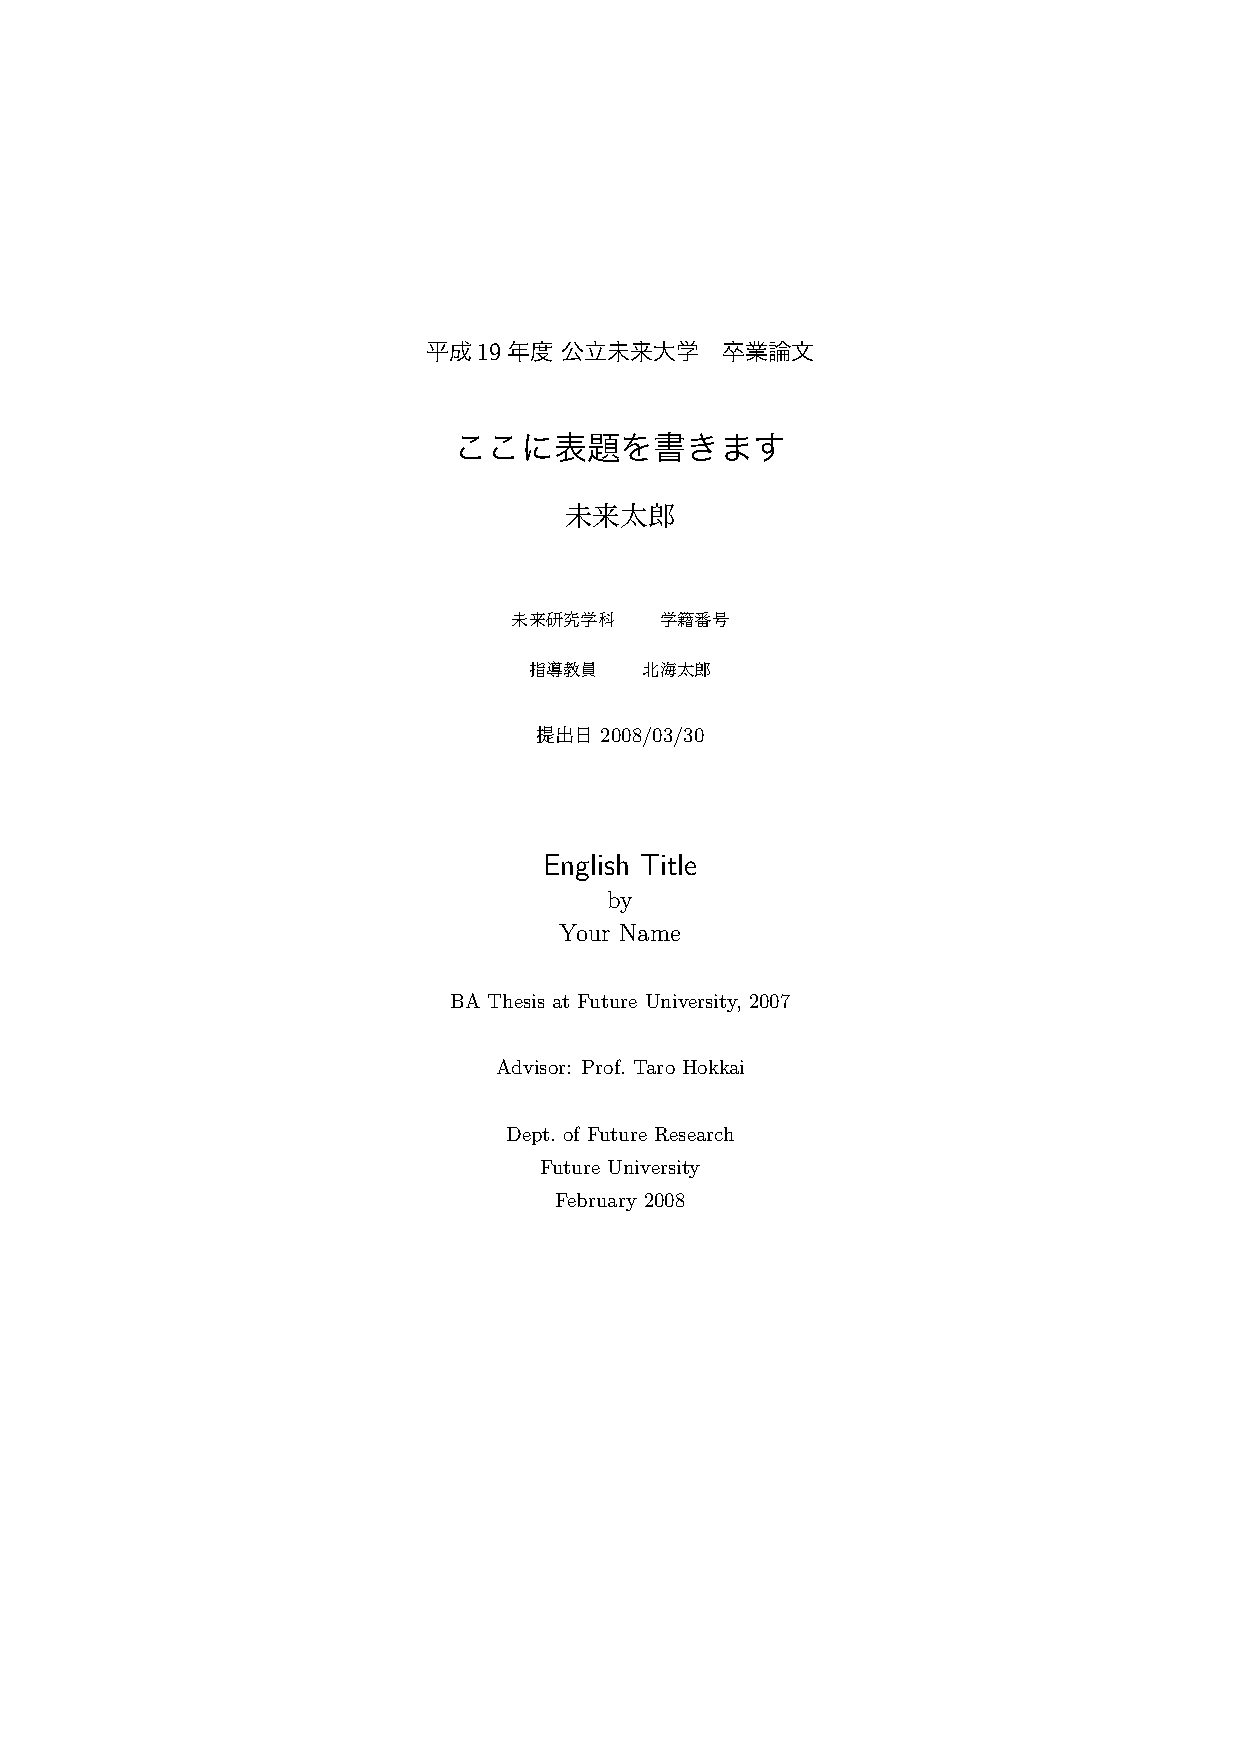
\includegraphics[scale=.75]{redef-title-smpl}}%
  \caption{表紙を手動で作成する例}
 \end{center}
\end{figure}

